\documentclass[10pt]{article}

\usepackage[margin=0.85in]{geometry}
\usepackage[T1]{fontenc}
\usepackage{lmodern}
\usepackage{microtype}
\usepackage{graphicx}
\usepackage{booktabs}
\usepackage{array}
\usepackage{amsmath,amssymb}
\usepackage{enumitem}
\usepackage[dvipsnames]{xcolor}
\usepackage[round,authoryear]{natbib}
\usepackage[colorlinks=true,allcolors=MidnightBlue]{hyperref}
\usepackage[nameinlink,noabbrev]{cleveref}

\setlist{nosep}
\graphicspath{{figures/}}
\hypersetup{
  pdftitle={GAWorld: Building Persistent and Situated LLM Agent Societies},
  pdfauthor={},
  pdfsubject={LLM-based artificial societies and multi-agent social simulation},
  pdfkeywords={LLM agents, multi-agent systems, artificial societies, social simulation}
}

\title{GAWorld: Building Persistent and Situated LLM Agent Societies}
\author{Author Name(s)\\Affiliation(s)\\\texttt{email@example.org}}
\date{2026}

\begin{document}
\maketitle

\begin{abstract}
LLM agents are increasingly used to study social interaction, yet many
demonstrations remain short-lived, weakly situated, or difficult to audit as
scientific instruments.  We present GAWorld, research infrastructure for
building persistent and situated LLM agent societies.  GAWorld connects
profile-grounded agents, structured state, file-backed memory, planning,
action, and reflection to a shared urban environment, social relations,
economic and work processes, information exposure, and controlled
interventions.  Its execution model combines a configurable cognition
pipeline with event and plugin boundaries while preserving compatibility with
directly integrated mechanisms during an incremental architectural migration.
The system exposes command-line, web, interview, replay, distributed
communication, and experiment-comparison interfaces, together with
heterogeneous artifacts that permit inspection from aggregate summaries back
to agent and subsystem traces.  We audit both the implementation and the
existing result archive, using memory, policy, information, and
economy--wellbeing cases to demonstrate research affordances and failure
visibility.  These artifacts establish system capabilities, not population
realism, causal policy effects, or prediction of real cities.  We therefore
frame GAWorld as a modular instrument for constructing and auditing artificial
society experiments, and make explicit the validation, reproducibility, and
ethical work required before stronger social claims are warranted.
\end{abstract}

\section{Introduction}
\label{sec:introduction}

Large language models (LLMs) make it possible to construct agents that
interpret natural-language situations, maintain plans, and generate socially
legible action.  This has renewed interest in generative agents and in using
LLMs to simulate individual or collective behavior
\citep{park2023generative,park2024grounded,argyle2023outofone}.  A convincing
conversation, however, is not yet an artificial society.  Society-level
research requires agents to persist across simulated time, act from locations
and relationships in a shared world, encounter consequences of earlier
actions, and leave evidence from which a researcher can reconstruct what
happened.  It also requires mechanisms outside the language model---time,
space, exposure, institutions, resource constraints, and interventions---to
remain explicit enough to inspect and vary.

These requirements create a systems problem.  Persistence cannot reside only
in a model context window: profiles, state, episodic experience, relationships,
and schedules must survive across ticks and runs.  Situatedness cannot be
reduced to scenery in a prompt: movement, co-location, local conditions, and
social ties must constrain later computation.  Experimental control requires
scenario configuration and intervention points that are distinct from the
agent's generated narrative.  Finally, scientific use requires provenance
below a polished transcript or aggregate plot.  A researcher should be able to
ask which mechanism produced a state change, whether every treatment
completed, and which model and configuration generated an archived trace.

GAWorld addresses this problem as research infrastructure for building
persistent and situated LLM agent societies.  It connects a continuing agent
lifecycle---profile, perception, memory and recall, planning and action,
reflection, state update, and storage---to an urban and societal substrate.
That substrate includes a city graph and local physical conditions, social
relationships and life events, economic state, work, information exposure,
and scheduled interventions.  A simulation clock and event boundaries connect
individual cognition to day-level and society-level evolution.  The resulting
unit of study is not an isolated model response but a configured run whose
local decisions, shared events, persistent state, and derived comparisons can
be inspected together.

The system is also an account of incremental research-software
modularization.  GAWorld began with tightly connected domain paths and is being
migrated toward a small execution kernel, configurable cognition stages, an
event bus, and lifecycle-managed plugins.  The current implementation contains
working examples of these boundaries while retaining direct calls, shared
dictionaries, subsystem-owned files, and hook-based compatibility paths.  We
document that mixed state rather than presenting an aspirational architecture
as complete.  This distinction is important for reuse and for science: a
mechanism that is configurable is not necessarily isolated, and an extension
that writes a metric is not necessarily on the causal path of an agent action.

This paper makes four contributions:

\begin{enumerate}[leftmargin=*]
  \item \textbf{A persistent and situated agent lifecycle.}  We describe how
  GAWorld joins relatively stable profiles, mutable structured state,
  file-backed memory, intentions, habits, relationships, interests, and skills
  to a configurable per-tick cognition pipeline and a shared simulation clock.
  The design makes continuity and context inspectable without treating them as
  evidence of psychological fidelity.

  \item \textbf{A composable urban-society substrate.}  We show how city,
  environment, social-network, economic, work, policy, and information
  mechanisms contribute to a common run.  Explicit coupling and provenance
  support experiments that cross individual and aggregate levels while making
  clear where calibration and mechanism validation remain necessary.

  \item \textbf{An extensible execution and research architecture.}  We
  present the configured stage pipeline, simulation context, event bus, plugin
  registry, controller and recorder skeletons, compatibility paths, and the
  command-line, dashboard, interview, replay, and relay interfaces built around
  them.  A migration-state audit separates wired services, partial
  integrations, and planned boundaries.

  \item \textbf{An inspectable experimentation workflow with bounded evidence.}
  We connect scenario configuration, matched-run comparison, structured
  artifacts, and GAWorld-Bench to an evidence ledger.  Existing memory,
  policy, information, and economy--wellbeing archives demonstrate what the
  system can record and expose; incomplete and diagnostic artifacts are
  reported alongside them rather than converted into claims of social
  validity.
\end{enumerate}

GAWorld is not presented as a digital twin, a representative synthetic
population, or a forecasting system.  Its current artifacts do not establish
that generated agents reproduce particular people, that aggregate trajectories
match a real city, or that a simulated intervention estimates a real policy
effect.  We instead treat the system as a scientific instrument whose outputs
must be evaluated at multiple levels and whose reproducibility is a prerequisite
for substantive interpretation.  This framing places software architecture,
experimental design, and validity boundaries in the same account.

The remainder of the paper proceeds from this distinction.  We first state
the design goals and position GAWorld relative to generative-agent,
language-agent, social-evaluation, and agent-based-modeling research.  We then
describe the agent lifecycle, execution architecture, memory and cognition,
and societal substrate.  Subsequent sections cover experiment and deployment
interfaces, audit the existing capability cases, and state the validation,
ethical, and development boundaries that govern intended use.

\section{Design Goals}
\label{sec:design-goals}

GAWorld is intended as a research instrument rather than a claim that a
language model is, by itself, a valid population model.  Its design goals
therefore concern properties that a researcher can inspect in the running
system.  Each property below has a concrete mechanism in the present
implementation and a boundary that prevents the mechanism from being read as
an empirical guarantee.

\subsection{Persistence across simulated time}

An agent should carry consequences from one decision context into later ones,
rather than being reconstructed from a stateless prompt at every tick.
GAWorld combines a mutable state record with file-backed episodic memory,
daily logs and diaries, schedules, and longer-lived relationship and growth
records.  A stateful run restores the day counter and per-agent memories, while
the memory lifecycle can retrieve, consolidate, summarize, and decay stored
episodes.  This makes persistence testable: a researcher can inspect both the
state before and after a tick and the files used in later recall.  Persistence
does not establish psychological fidelity.  Several memories and summaries
are language-model outputs, configuration can disable lifecycle operations,
and the archived cross-phase evaluation discussed later in the paper is
incomplete.

\subsection{Situatedness in a shared world}

Actions should be conditioned on where and when an agent acts and on what is
locally observable.  The simulation clock exposes day, time, and tick index;
the city map represents named locations and connections; and environment,
local-physical, social, policy, and information mechanisms contribute context
to the cognition loop.  Movement updates location before later stages use the
new setting, and social influence is computed over the current network rather
than over an unconstrained cast of characters.  This is situated computation,
not a calibrated digital twin: map detail, physical dynamics, and agent access
to information are abstractions selected by configuration.

\subsection{Composability without concealing control flow}

Researchers should be able to change an experimental mechanism without
rewriting the complete agent loop.  GAWorld provides three bounded extension
surfaces: a configurable stage sequence for cognition, an event bus with
observe/contribute/filter semantics, and a registry for lifecycle-managed
plugins.  The audited built-in set contains nine plugins: interventions,
skills, interests, life events, economy, local physical perception, real work,
dynamic behavior, and spatial preferences.  Composability is not unrestricted
hot swapping: stages exchange a shared dictionary, while memory, environment,
and social-network logic retain direct compatibility paths.

\subsection{Controllability for counterfactual experiments}

A research run should expose explicit points at which a scenario or
intervention is introduced.  Configuration fixes profiles, city assets,
random seed, mechanism flags, schedules, and policy events; the intervention
plugin contributes a recommendation feed through the event bus and records
its domain-specific metrics.  Baseline/event workflows can then align traces
produced under different scenario specifications.  The kernel also defines a
Controller API for validators and named runtime interventions.  Structured
movement requests pass through its validator chain, and the standard runtime
interventions update agent state, update live configuration, or queue agent
removal with audit records.  Other selected actions are not universally
mediated, so configuration, scheduled events, hooks, and experiment scripts
remain important control surfaces.

\subsection{Inspectability from decision to artifact}

A claim about an artificial society should be traceable to artifacts below the
level of a prose summary.  GAWorld writes per-agent logs and memories,
environment timelines, state histories, plugin-owned outputs, and experiment
comparisons; its interfaces expose portions of those records for inspection
and replay.  The kernel Recorder additionally implements a clock-stamped JSONL
stream and records Controller interventions and denials.  That unified stream
is not yet the main action/trace path: the established simulator continues to
write several specialized formats directly.  Inspection therefore requires
an artifact ledger that names the producing path and schema, and replayability
must not be inferred merely from the presence of logs.

\subsection{Backward-compatible modularization}

The system must remain usable while a monolithic research prototype is
decomposed.  A typed \texttt{Agent} view shares, rather than copies, the legacy
dictionary; \texttt{EventBus} preserves the legacy hook signature; and the
12-stage pipeline was carved from the existing per-agent step while retaining
the shared step dictionary.  These adapters allow migrated and legacy modules
to coexist and make migration state observable.  They also retain weakly typed
surfaces and shared mutable state.  Backward compatibility is thus a transition
strategy, not evidence that modularization is complete or that every old
configuration produces an identical trajectory.

\section{Related Work}
\label{sec:related-work}

GAWorld draws on four bodies of work that answer different parts of the
artificial-society problem.  Its contribution is a system integration and an
audited set of research surfaces; we do not claim that the underlying ideas of
memory, tool-using agents, social evaluation, or agent-based validation are
unique to GAWorld.

\subsection{Generative agents and simulated individuals}

Generative Agents demonstrated that an LLM-driven architecture combining an
experience stream, retrieval, reflection, and planning can sustain socially
legible behavior in a sandbox community \citep{park2023generative}.  That work
provides a central precedent for persistent social characters and for studying
emergent interaction through an inspectable environment.  Later work grounds
agents in extensive self-report data and evaluates how well responses predict
held-out answers from the same individuals \citep{park2024grounded}.  Research
on ``silicon samples'' similarly explores conditioning language models to
approximate distributions of survey responses
\citep{argyle2023outofone}.  These studies motivate profile grounding and
longitudinal state, but they also distinguish two validation targets:
internally coherent simulated inhabitants and externally evaluated models of
particular people or populations.

GAWorld is oriented toward constructing the surrounding research system.  It
adds configurable urban, social, economic, work, information, and policy
mechanisms; multiple operational interfaces; and explicit experiment and
artifact workflows around a persistent-agent loop.  Its archived profiles and
traces have not undergone the held-out, person-level validation used in work
on self-report-grounded agents.  Accordingly, GAWorld adopts persistence as a
system property and treats fidelity as an open empirical claim.

\subsection{Language-agent cognition and architecture}

LLM-agent research has developed reusable patterns for coupling language
generation to action.  ReAct interleaves reasoning and environment-facing
actions \citep{yao2023react}; Reflexion stores verbal feedback to improve later
attempts \citep{shinn2023reflexion}; and Voyager combines iterative prompting,
environment feedback, and an accumulating skill library in an open-ended
embodied setting \citep{wang2023voyager}.  MemoryBank studies long-term memory
with retrieval and forgetting mechanisms \citep{zhong2024memorybank}, while
CoALA offers a conceptual organization of language agents in terms of memory,
action space, and decision procedures \citep{sumers2024coala}.  CAMEL, in
turn, examines role-conditioned communication among language agents
\citep{li2023camel}.

These systems and abstractions inform GAWorld's separation of structured
state, episodic storage, retrieval, planning, action, reflection, and learned
skills.  GAWorld differs in scope rather than by proposing a new generic
reasoning algorithm: it connects such components to a persistent multi-agent
society and to a clocked, file-backed experimental runtime.  Its twelve-stage
pipeline, event bus, and plugin registry expose replacement and observation
points, but the present migration remains mixed with direct and hook-based
paths.  Thus GAWorld contributes an implemented integration for social
simulation, not a claim of a universally superior cognitive architecture.

\subsection{Social-agent tasks and evaluation}

AgentBench evaluates LLM agents across interactive environments and emphasizes
the gap between language ability and reliable action
\citep{liu2024agentbench}.  AgentBoard adds fine-grained progress measures and
analytical visualization for multi-turn agents \citep{ma2024agentboard}.
SOTOPIA focuses specifically on social intelligence by placing agents in
interactive social scenarios and evaluating goal achievement and social
dimensions \citep{zhou2024sotopia}.  Together, these benchmarks provide
controlled tasks, comparative evaluation, and diagnostics for an agent or a
small interaction.

GAWorld addresses a complementary unit of analysis: a persistent society run
whose agents, environment, institutions, and artifacts evolve across simulated
time.  Its benchmark layer can check selected outputs, known-sign diagnostics,
placebos, and determinism when suitable artifacts exist, but it is not a
replacement for standardized social-intelligence or interactive-agent
benchmarks.  Conversely, task success alone does not validate population
composition, emergent dynamics, or policy counterfactuals.  GAWorld therefore
retains agent-level traces and run-level evidence status so that task
competence, social interaction, and society-level claims can be evaluated
separately.

\subsection{Agent-based social simulation and validation}

Agent-based modeling (ABM) treats macro patterns as outcomes of specified
micro-level rules and interactions, while generative social science emphasizes
using such models to explain how collective regularities can arise
\citep{epstein2006generative}.  The ODD protocol provides a standard vocabulary
for documenting an individual- or agent-based model's overview, design
concepts, and details \citep{grimm2006odd}.  Methodological work on empirical
ABM validation stresses that matching selected aggregate observations is not
sufficient: calibration, identification, sensitivity, multiple validation
targets, and out-of-sample evidence remain distinct concerns
\citep{windrum2007empirical,fagiolo2007critical}.

GAWorld inherits this demand for explicit mechanisms and layered evidence, but
LLM mediation introduces additional sources of variation.  Prompt context,
provider behavior, model versions, parsing fallbacks, and generated text can
change trajectories even when conventional parameters and seeds are recorded.
The system therefore couples ABM-style configuration and intervention design
to provider logs, raw agent traces, per-arm completion status, and an artifact
ledger.  Its present archive supports software-path and affordance claims, not
empirical validation of a population model.  This distinction also responds to
concerns that language models should not be treated as drop-in replacements
for human participants \citep{dillion2023replace}, particularly when generated
outputs can flatten variation within identity groups
\citep{wang2025flatten}.

\section{Persistent and Situated Agent Lifecycle}
\label{sec:agent-lifecycle}

GAWorld represents an agent as a continuing participant in a shared simulation,
not as an isolated chat session.  The representation separates relatively
stable profile material, mutable runtime state, and artifacts accumulated over
simulated time.  Figure~\ref{fig:agent-lifecycle} shows the connected per-tick
control path.

\begin{figure}[t]
  \centering
  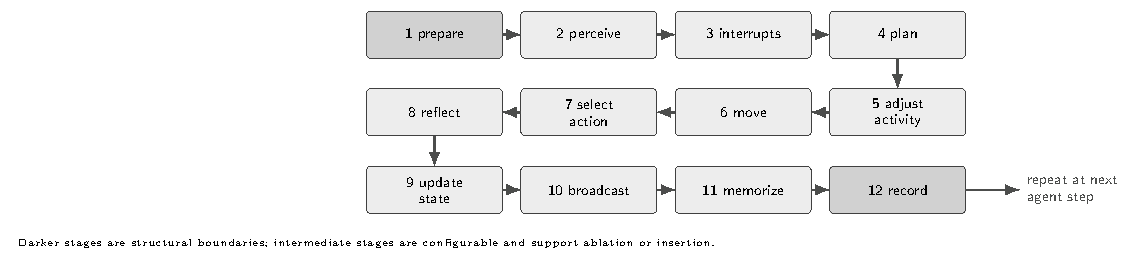
\includegraphics[width=\linewidth]{agent_lifecycle.pdf}
  \caption{The configured default agent-step pipeline.  The first and last
  stages are structural boundaries; intermediate stages may be omitted or
  replaced through configuration.  Domain inputs also arrive through direct
  calls and event-bus contribution points, so the diagram is a control-flow
  account rather than a claim that every subsystem is a plugin.}
  \label{fig:agent-lifecycle}
\end{figure}

\subsection{Profile seeds and mutable state}

At construction time, a tabular seed row supplies the identifier,
demographic fields, and initial scalar state, while a Markdown profile supplies
descriptive material such as occupation, personality, daily life, and values.
The current builder merges these sources into a dictionary containing
\texttt{id}, profile fields, \texttt{state}, an in-memory \texttt{memory}
list, and \texttt{social\_neighbors}; it then initializes location against the
city map.  The core state includes affective, socioeconomic, identity,
behavioral, and information-exposure variables.  Additional mechanisms may
add namespaced or compatibility fields during setup and execution.

The class \texttt{gaworld.core.agent.Agent} is a typed adapter over this
dictionary.  It provides properties for identifier, name, state, memory,
schedule, location, and attached skill identifiers, while dictionary access
delegates to the same backing object.  \texttt{view\_as\_agent} therefore
introduces no copy, and \texttt{ensure\_agent\_dict} allows a typed caller to
hand the record back to older helpers.  This is important for incremental
migration, but it is not a fully typed agent schema: many runtime call sites
still consume dictionaries, and arbitrary mechanism-specific fields can still
be added.

Persistence extends beyond the in-memory record.  Depending on enabled
features, per-agent directories hold episodic entries, diaries, schedules,
vector-indexed recall material, environmental preferences, and other
mechanism-owned records.  On a stateful restart, stored memory is loaded into
the agent and can seed retrieval.  The file boundary makes inputs to later
decisions inspectable, although it also means that reproducibility depends on
capturing configuration, external model behavior, and the complete artifact
directory rather than only the seed CSV.

\subsection{The default per-tick path}

The cognition loop is implemented as an ordered \texttt{StagePipeline}.  A
stage receives an agent, a shared per-step dictionary, and the
\texttt{SimContext}.  Hook-visible values retain names such as
\texttt{activity}, \texttt{action}, \texttt{outcome}, and
\texttt{reflection}; intermediate values use underscore-prefixed keys.  The
default path contains the following twelve stages:

\begin{enumerate}[leftmargin=*,label=\arabic*.]
  \item \textbf{prepare} establishes tick-local inputs and emits the pre-step
  boundary;
  \item \textbf{perceive} combines local environment, social, policy, memory,
  and contributed perception sections;
  \item \textbf{interrupts} considers events that can alter the scheduled
  course;
  \item \textbf{plan} forms the agent's immediate intention in the current
  context;
  \item \textbf{adjust\_activity} reconciles that plan with scheduled and
  interrupted activity;
  \item \textbf{move} resolves travel and updates location where applicable;
  \item \textbf{select\_action} chooses an action from the available action
  space;
  \item \textbf{reflect} produces an interpretation of action and outcome;
  \item \textbf{update\_state} applies state and relationship effects;
  \item \textbf{broadcast} exposes eligible communication to other agents or
  a distributed relay;
  \item \textbf{memorize} constructs and stores the tick's experience; and
  \item \textbf{record} appends established logs, state history, and visual
  trace material.
\end{enumerate}

Before the pipeline runs, the outer loop advances the shared Clock, updates the
environment and local occupancy, polls distributed messages when enabled, and
may perform configured information seeking.  After it returns, the runtime
emits \texttt{on\_agent\_post\_step}, allowing mechanisms such as the
intervention plugin to compute their own metrics.  Day-start and day-end
events bracket the tick loop, and memory consolidation is invoked at the end
of a day.  Consequently, the twelve stages are the agent-step spine, not the
entire simulation lifecycle.

\subsection{Contribution points and compatibility calls}

The EventBus lets a mechanism observe an event, contribute zero or more items,
or filter a value in priority order.  Perception composition is a concrete
example: local context can be assembled by established code while plugins add
bounded text sections without owning the full prompt.  Post-step and day-end
events similarly let policy, economy, skills, or interests react at defined
boundaries.  Observer failures are logged and isolated unless strict mode is
enabled; stage failures instead propagate because a missing control-flow stage
could silently corrupt state.

Not all inputs use this bus.  Memory recall, environment evolution, and social
network operations retain direct paths within or around the pipeline.  The
Controller now validates structured movement requests and exposes audited
runtime interventions, but it does not mediate every selected action.
Likewise, \texttt{record} writes established artifacts in addition to the
kernel Recorder.  The lifecycle is therefore connected and configurable while
retaining compatibility paths beyond the plugin boundary.

\subsection{Configuration and ablation semantics}

The stage order is read from \texttt{CONFIG["pipeline"]["agent\_step"]}.
Entries may name built-in stages or importable callables; a custom callable can
also receive a display name.  Unresolvable entries are skipped with a warning,
and an empty resolved pipeline is rejected.  Downstream built-ins generally
read absent step values defensively, which supports mechanism ablations, but
\texttt{prepare} and \texttt{record} are intended as structural boundaries.
Changing order or removing a stage can change semantics and artifact
completeness.  The configuration surface therefore enables controlled system
experiments; it does not guarantee that every permutation is meaningful or
behavior-preserving.

\section{Execution Architecture and Incremental Modularization}
\label{sec:execution-architecture}

GAWorld combines a connected cognition pipeline with a small kernel, nine
built-in plugins, and compatibility-preserving domain paths.
Figure~\ref{fig:system-architecture} freezes the audited K1--K5 runtime at
repository commit \texttt{35a551e}.  The archived capability cases predate
this migration and are not evaluations of it.

\begin{figure}[t]
  \centering
  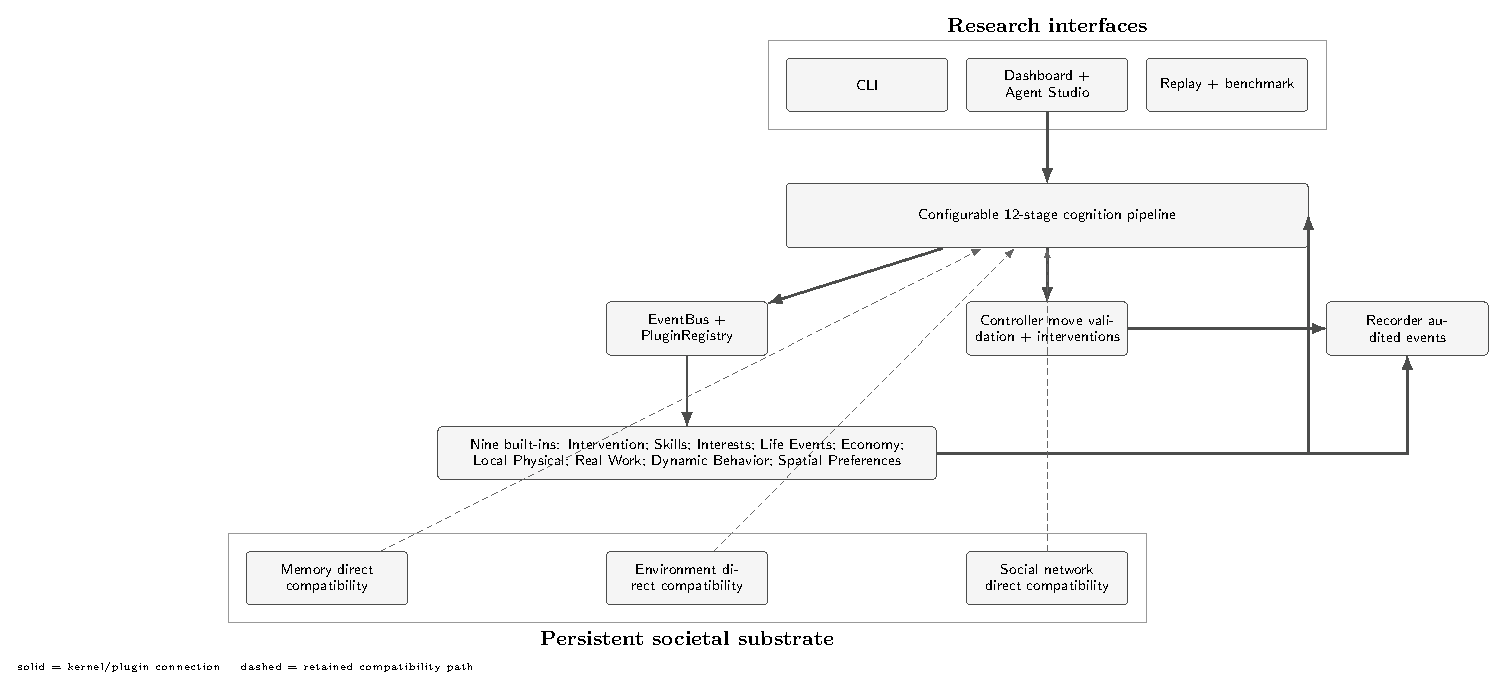
\includegraphics[width=\linewidth]{system_architecture.pdf}
  \caption{Audited execution architecture at commit \texttt{35a551e}.  Nine
  built-ins contribute through the registry, bus, pipeline filters, or
  lifecycle events.  Movement uses the Controller validation gate; Recorder
  events coexist with established domain-specific outputs.}
  \label{fig:system-architecture}
\end{figure}

\subsection{Kernel services}

\paragraph{Simulation context and clock.}
\texttt{SimContext} holds configuration, Clock, EventBus, PluginRegistry,
Controller, Recorder, agents and their identifier index, an LLM callable, a
seeded random-number generator, and an \texttt{extras} compatibility escape
hatch.  It also provides simulation-level and per-agent plugin-state
namespaces.  The outer loop is the sole clock writer, giving stages, plugins,
and records a common simulated day, time, and tick.  This ordering does not by
itself make model calls, external services, or concurrency deterministic.

\paragraph{Event bus and plugin registry.}
The EventBus supports priority-ordered observation (\texttt{emit}), merged
contribution (\texttt{collect}), and value rewriting (\texttt{filter}).
Handler failures are logged and isolated by default, so warnings and active
plugin lists must accompany results.  The PluginRegistry assembles built-ins,
configuration-named classes, and installed entry points; orders setup by
declared dependencies; skips failed or unsatisfied plugins; and tears active
plugins down in reverse order.  Plugins may own configuration, namespaced
agent state, and output directories, but execute in process and are not a
sandbox.

\paragraph{Controller.}
The Controller provides a priority-ordered validator chain over structured
\texttt{ActionRequest}s and a named runtime-intervention API.  In the main
simulator, movement requests pass through validation: denial preserves the
origin and is surfaced in the next perception, while a rewrite can change the
destination.  K5 registers standard interventions for setting one agent-state
value, updating a dotted live-config path, and queueing agent removal for the
next day boundary.  Denials and interventions are audited through the
Recorder.  Other selected actions are not all mediated, so the Controller is
not a universal policy or safety gate.

\paragraph{Recorder.}
The Recorder appends clock-stamped JSON objects to table-specific files and is
closed when the simulation exits.  It records Controller activity and is
available to plugins.  Main traces, state history, memories, environment
events, and specialized metrics also retain established writers.  Recorder
integration therefore improves cross-plugin auditability without implying
that the archive can be replayed from one event log.

\subsection{Built-in plugin assembly}

The audited registry assembles Intervention, Skills, Interests, Life Events,
Economy, Local Physical, Real Work, Dynamic Behavior, and Spatial Preferences.
They attach domain behavior to day/tick events, perception contributions,
location filters, action or outcome filters, and post-step or day-end hooks.
For example, Intervention contributes recommendation context and persists
policy metrics, Life Events produces scheduled exogenous events and state
effects, Local Physical contributes nearby conditions, and Spatial Preferences
can rewrite a resolved destination.  The adapters delegate calculations and
specialized persistence to established modules: migration changes
orchestration and ownership, not the scientific validity of the mechanisms.

\subsection{Migration-state audit}

\begin{table}[t]
\centering
\small
\setlength{\tabcolsep}{4pt}
\begin{tabular}{@{}p{0.17\linewidth}p{0.23\linewidth}p{0.19\linewidth}p{0.32\linewidth}@{}}
\toprule
Surface & Current boundary & Status & Retained boundary and consequence \\
\midrule
Cognition & Configured 12-stage pipeline & Wired & Shared step dictionary; order and omissions must be reported \\
Extensions & EventBus and PluginRegistry & Wired & Failures may degrade rather than terminate a run \\
Nine domain adapters & Policy, skills, interests, events, economy, physical, work, behavior, spatial & Plugin-integrated & Established stores and writers remain; activation needs config/plugin provenance \\
Memory & Recall, storage, consolidation, decay & Direct compatibility path & Persistent context is inspectable, not psychologically validated \\
Environment and social network & World evolution and network modules & Direct compatibility path & The full world and network models are not isolated plugins \\
Controller & Move validation and named interventions & Connected, scoped & Other actions retain established paths; no universal-gate claim \\
Recorder & Clocked structured event writer & Connected, non-exclusive & Multiple writers remain; no single-log replay claim \\
\bottomrule
\end{tabular}
\caption{Implementation state in the audited repository.  K1--K5 completion
does not imply that every subsystem or output format is isolated.}
\label{tab:migration-state}
\end{table}

\subsection{Failure and reproducibility boundaries}

A cognition-stage exception propagates because the stage is control flow.
Bus-handler and plugin-setup failures instead warn and normally leave the
remaining run active; missing dependencies deactivate the affected plugin.
Operational resilience therefore makes a completed process different from a
complete treatment.  A reproducible artifact must include resolved stage
order, active plugin identifiers, warnings, configuration, source snapshot,
model/provider conditions, and specialized outputs.

The scoped K1--K5 migration is complete, but shared dictionaries, the context
escape hatch, direct domain calls, and multiple recording paths remain.
``K1--K5 complete'' describes completion of the migration plan, not universal
subsystem isolation or validation.

\section{Memory, Cognition, and Behavioral Continuity}
\label{sec:memory-cognition}

GAWorld separates persistence from generation.  An agent's continuity is not
held solely in an LLM context window: structured state, episodic records,
habits, intentions, relationships, environmental preferences, growth profiles,
and skills are written to mechanism-specific stores and reintroduced at later
steps.  Figure~\ref{fig:memory-growth} summarizes this path.  The resulting
system can preserve and expose information across simulated days; whether its
memory dynamics resemble those of people is a separate empirical question.

\begin{figure}[t]
  \centering
  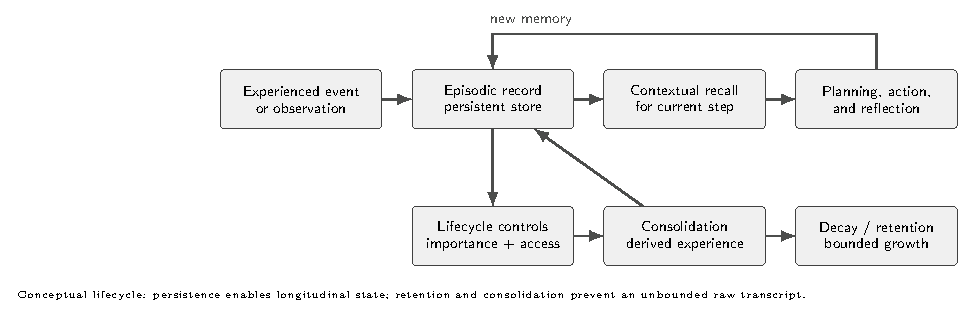
\includegraphics[width=0.94\linewidth]{memory_growth.pdf}
  \caption{Persistent experience and growth paths.  Tick-level episodes feed
  retrieval and rule-based updates; configured day-boundary processes may
  consolidate episodes into semantic memories or private skills.  Solid
  storage paths denote implemented persistence, not validated models of human
  remembering or learning.}
  \label{fig:memory-growth}
\end{figure}

\subsection{Episodic persistence and retrieval}

The basic store retains an agent's memory list, schedule, available actions,
locations, and location--action biases as JSON, alongside append-only textual
logs and simulation state.  A second experience layer records episodes in
JSONL and persists habits, daily intentions, relationships, and environmental
preferences in separate per-agent files.  This division supports inspection
and selective restart, although a complete restart requires all of these
stores rather than a single canonical agent file.

For content-addressed recall, memory entries are also indexed in SQLite with
type, simulated time, salience, recall count, and an embedding.  The configured
embedding path may call an embedding provider; if that path is unavailable,
the implementation falls back to a deterministic hash embedding.  Retrieval
combines vector similarity with salience, age decay, and prior recall, then
optionally boosts entries related to the agent's current growth interests.
Thus ranking is a specified scoring procedure over stored entries, whereas the
text being ranked may have originated in an LLM-generated action, reflection,
diary, news item, or external source.

The day-boundary lifecycle adds two optional transformations.  Consolidation
selects recent episodic rows and asks an LLM to distill them into a small set of
semantic entries; malformed output or insufficient material produces no new
entry.  Decay is LLM-free: after a configured period it lowers the salience of
old, unrecalled episodic rows and deletes rows already below a floor, while
protecting semantic, external-information, and procedural entries.  A separate
episode store also computes exponential salience decay and enforces a size cap.
These two decay paths operate over different stores and should not be mistaken
for one unified cognitive theory.

External retrieval-augmented memory is likewise optional.  Agent-derived
queries can retrieve web material, after which an LLM may assess or compress
it into external-information entries.  This path depends on a caller-supplied
fetch adapter and degrades to no operation on failure.  Consequently, an
experimental report must disclose whether external retrieval, provider-based
embeddings, consolidation, and decay were enabled.

\subsection{Intentions, habits, and reactive behavior}

Behavioral continuity combines model-mediated interpretation with explicit
state-transition rules.  At day boundaries, recent episodes and current state
can be supplied to an LLM to produce priorities, avoidances, social targets,
and recovery goals.  When the call budget is exhausted or parsing fails, a
rule-based fallback constructs intentions from state and recent experience.
Habit strength, relationship signals, physiological and time-pressure needs,
episode salience, and many mood or stress adjustments are updated by bounded
numeric rules.  These values enter subsequent prompt context rather than being
left as unstructured prose.

The dynamic-behavior module evaluates candidate interruptions from needs,
co-location, incoming messages, environmental events, local physical
conditions, cascades, and spontaneous urges.  Acceptance probabilities depend
on event intensity, activity commitment, personality proxies, relationship
closeness, and agent state.  Candidate generation and schedule insertion are
LLM-free but stochastic; they are repeatable only when the relevant random
state is seeded.  Once an interruption wins, the ordinary activity-adjustment
or action path may invoke an LLM to phrase or refine the response.  GAWorld
therefore distinguishes rule-based opportunity and constraint generation from
model-generated interpretation and action text.

Spatial preference illustrates continuity without language generation.  A
crowd surge or other location anomaly raises a time-bucketed aversion score;
scores decay with recency, and a later destination can be redirected when its
aversion crosses a configured threshold.  This mechanism implements learned
avoidance as a transparent rule.  It does not establish that the learning rate,
threshold, or decay reproduces human spatial choice.

\subsection{Interests, skills, and productive activity}

Growth profiles contain bounded hobby and skill items with phase, engagement,
competence, practice history, and activity templates.  Their initial content
may be derived by an LLM and cached by a profile signature; deterministic
fallback profiles are available when generation fails.  Episode matching,
practice updates, phase classification, daily retention decay, retirement of
stale interests, and socially mediated adoption then use explicit rules and a
seedable random generator.  The labels borrow a developmental vocabulary, but
their implementation is a simulation mechanism rather than a validated model
of human interest development.

The skill subsystem maintains a curated global library and per-agent private
skills.  Available skills can be injected into cognition context, while an
optional LLM consolidation step extracts a reusable procedure from recent
episodes and saves it as a private Markdown skill.  Parsing, schema checks, and
registry precedence constrain this output; they do not demonstrate that the
procedure is correct or transferable outside the generated setting.

Productive activity extends this pattern to a mock work market.  Cached,
LLM-derived capability profiles and current growth items inform routing.  A
JSONL queue provides claim and recovery semantics, a worker pool dispatches
briefs concurrently, and code, content, teaching, and web-design adapters use
an LLM to produce files.  Lightweight validators check properties such as
Python syntax, Markdown structure, or HTML/SVG parseability before successful
results are ingested into agent state and market settlement.  These checks and
persisted artifact paths demonstrate a functioning production pipeline; they
are not evidence that an artifact meets professional, pedagogical, factual, or
security standards.

\section{Situated Urban and Societal Substrate}
\label{sec:societal-substrate}

GAWorld places persistent agents in a shared substrate whose components read
and write overlapping state.  The city constrains movement, local occupancy
changes perception, relationships affect encounters, and financial or life
events alter later choices.  This coupling supports questions that cross
individual and aggregate levels, but it also means that mechanism provenance
and configuration are part of every experimental treatment.

\subsection{City graph and local physical conditions}

The city map parses places, roads, transit lines, interiors, and land-use
attributes into a graph.  Nodes carry categories, coordinates, capacity,
opening hours, popularity, density, and display metadata.  Destination
resolution can match activity terms to place categories, while graph routing
and transport-mode rules estimate distance, time, and fare.  Mode speeds,
fixed delays, road-class multipliers, rush-hour penalties, area price levels,
and weather preferences are explicit parameters.  They make travel costs
inspectable; their presence does not imply transport-model calibration.

At each tick, the local-physical layer recomputes occupancy from stationary
agents, clears stale counts, and exposes the current location's crowding,
opening status, and weather.  A crowd anomaly is flagged when occupancy is both
high and sharply above the previous tick.  These snapshots can enter
perception and interruption generation, linking collective movement to
individual behavior.  The mechanism is deterministic given agent locations
and parameters, although the locations themselves may follow stochastic or
LLM-mediated decisions.

The broader environment system supports configured natural, economic,
political, technological, and intraday events.  In rule mode it samples from
configured event distributions using a local random generator.  In LLM mode a
model proposes a daily summary, events, and intraday rules that are parsed into
the same bounded event schema; configured fallback generation remains
available if that call fails.  Severity and anomaly tagging are rule-based.
Reports must therefore identify the generator mode rather than treating all
environmental histories as equivalent.

\subsection{Social ties and life events}

Relationships are typed records rather than undifferentiated neighbor edges.
Role templates specify channels, obligation, protection, and daily decay;
interaction signals update closeness and contact time.  The implementation can
bootstrap off-screen contacts from an LLM-generated backstory, with a
deterministic heuristic fallback.  It can also generate events involving
off-screen contacts, using templates and optional LLM wording, and disclose
shared contacts across agents.

Maintenance is rule-based.  Uncontacted ties decay at role-specific rates,
long-neglected obligations can rise, and an enforcement pass assigns nested
Dunbar-style tiers while pruning beyond a configured outer cap and protecting
selected kin roles.  These tiers are an operational capacity constraint, not
evidence that the simulated network reproduces measured human networks.

Life events are normalized, persisted, scheduled by simulated day and time,
and drained once when due.  Events can target agents and carry bounded state
effects and tags.  This provides a controlled exogenous-event surface whose
timing and direct updates are inspectable.  The realism of event frequencies,
dependencies, and consequences must be established by a separate study.

\subsection{Economic state transitions}

The finance module maintains checking, savings, investment, and housing-fund
accounts; monthly budgets; income and expense records; liabilities and credit;
sector pools; government flows; and macro state.  Configured rules calculate
social-insurance deductions and progressive income tax, route wages and
consumption, enforce available-cash and credit constraints, transfer savings,
and settle payments.  A dedicated seeded random generator drives expenditure
variation, market returns, shocks, and other probabilistic transitions so that
unrelated random draws need not perturb the economy sequence.

Shared sector and government pools make counterparties visible instead of
creating every monetary flow without an account.  Agent-to-agent payments and
some rent or labor flows can be routed to modeled recipients; investment
returns combine a common market component with idiosyncratic variation.
Ledger and conservation checks can reveal implementation defects such as
unbalanced internal transfers.  They cannot establish that the tax schedule,
consumption response, labor process, credit behavior, or macro dynamics is an
empirically valid representation of a real economy.  Accounting consistency
is therefore a software invariant, not a behavioral-validation result.

\subsection{Coupling and ownership boundaries}

Table~\ref{tab:component-coupling} makes the principal shared-state paths
explicit.  ``Implemented'' refers to an inspectable current mechanism;
``partial boundary'' indicates that the mechanism is connected but retains
direct calls, shared dictionaries, or specialized writers rather than a fully
isolated plugin interface.

\begin{table}[t]
\centering
\small
\setlength{\tabcolsep}{3.5pt}
\begin{tabular}{@{}p{0.14\linewidth}p{0.17\linewidth}p{0.17\linewidth}p{0.27\linewidth}p{0.16\linewidth}@{}}
\toprule
Subsystem & Reads & Writes & Agent-visible consequence & Evidence status \\
\midrule
Memory and cognition & Episodes, state, context, retrieved entries & Memories, intentions, habits, relationships & Recalled context, priorities, reflection, and later action bias & Implemented; human realism unvalidated \\
Interests and skills & Profile, episodes, social growth context & Growth profile, private skills & Practice focus and procedural prompt context & Implemented; partial plugin boundary \\
World and local physics & City graph, time, weather, locations & Routes, travel state, occupancy snapshots & Feasible destinations, travel costs, crowding and closure cues & Implemented; direct integration \\
Environment & Configuration, history, optional LLM output & Events, weather and macro context & Interruptions and perceived exogenous conditions & Implemented; generator-mode dependent \\
Social network & Profiles, contact history, interactions & Typed ties, closeness, obligation, tiers & Encounter probability and relationship context & Implemented; mechanism validity unassessed \\
Life events & Persisted event queue, clock & Consumption flag and configured state effects & Scheduled exogenous changes to targeted agents & Implemented; committed plugin-integrated event producer \\
Economy & Activity, balances, calendar, sectors, macro state & Accounts, ledger, budgets, pools, agent state & Income, spending constraints, taxes, credit, returns and payments & Implemented; primarily hook-based \\
Work & Capability cache, activity, growth, market jobs & Queue results, artifacts, settlement and state effects & Produced files, earnings, and experience records & Implemented; artifact quality unvalidated \\
\bottomrule
\end{tabular}
\caption{Coupling among agent and societal components.  Evidence status
describes implementation visibility, not empirical validity.}
\label{tab:component-coupling}
\end{table}

The table also exposes the current modularity limit.  Interests and skills have
plugin entry points, and economy, local physical perception, spatial
preferences, work, and dynamic behavior now have built-in adapters.  Memory,
environment evolution, and social-network operations still exchange mutable
agent dictionaries or runtime objects directly.  This arrangement is usable
and inspectable, yet replacing
one mechanism can change prompts, state schemas, random draws, and specialized
artifacts elsewhere.  Controlled comparisons should therefore freeze the
complete coupled configuration rather than naming only the focal intervention.

\section{Experimental Workflow and Evidence Production}
\label{sec:experiment-workflow}

GAWorld treats an experiment as a configured execution that produces an
inspectable artifact tree, rather than as a prompt followed by a single model
response.  The ordinary entry point, \texttt{generative\_city\_sim.py run},
loads the selected agents and city map, restores persistent state when enabled,
assembles the currently integrated plugins, and advances a shared simulation
clock.  Runtime configuration controls the horizon, agent cohort, random seed,
provider routing, environment, policy events, and output locations.  A run can
therefore be reconstructed at the level of its declared configuration and
stored traces, although exact replay also depends on external model behavior,
network services, and the completeness of the archived inputs.

\subsection{Matched Event and Baseline Runs}

For intervention studies, the \texttt{compare-event} command constructs two
scenario directories under a timestamped comparison root.  The
\texttt{without\_event} arm inherits the configured policy-event list, whereas
the \texttt{with\_event} arm appends a named event at an explicit simulation
day and clock time.  Both arms receive the same requested agent subset,
simulation horizon, random seed, and---when supplied---LLM provider override.
Before execution, each arm is reset within its own isolated memory, log,
vector-database, state, network, environment, intervention, and visualization
directories.  The two runs are then launched concurrently.  This organization
reduces accidental cross-arm state leakage and makes missing or failed arms
visible through separate reset and run logs.

After both subprocesses finish, the comparison routine reads each arm's
\path{state/agent_state_history.csv}.  For every available metric, it
computes the across-agent final snapshot, the mean over recorded observations,
and event-minus-baseline differences.  Machine-readable results are stored in
\path{comparison_metrics.csv}; \path{comparison_summary.md} provides a
human-readable view.  The separate \path{run_meta.json} records choices such
as seed, horizon, provider, and whether the lower-fidelity fast mode was
requested.  Policy-oriented fields can include stance, toxicity,
misinformation risk, cross-viewpoint exposure, and intervention reward when
their upstream mechanisms emit them.  Importantly, archived policy runs contain
fields that remain identically zero, including misinformation-risk and
cross-viewpoint-exposure series in some comparisons.  Presence in the schema
must therefore not be reported as evidence that the corresponding mechanism was
active.

\begin{figure}[t]
  \centering
  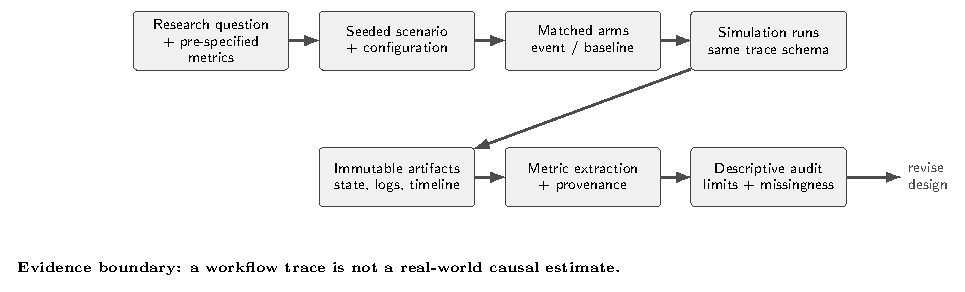
\includegraphics[width=\linewidth]{experiment_flow.pdf}
  \caption{GAWorld's experiment path separates a research question and
  configured scenario from matched execution arms, stored traces, metric
  extraction, and a descriptive audit.  The final boundary is substantive:
  an inspectable comparison is not by itself a real-world causal estimate.}
  \label{fig:experiment-flow}
\end{figure}

\subsection{What Matching Does---and Does Not---Identify}

Sharing a pseudorandom seed and configuration is a software control, not a
causal-identification strategy.  LLM endpoints can be nondeterministic despite
fixed sampling parameters; concurrent calls may experience different failures,
fallbacks, latency, or service-side model revisions; and an injected event can
change subsequent prompts and thereby amplify trajectory divergence.  Moreover,
the implemented report contrasts raw trajectories without random assignment,
replication, uncertainty estimation, or adjustment to an external population.
Consequently, GAWorld's paired output supports debugging, mechanism tracing,
and hypothesis generation.  It does not establish that a measured difference
was caused by the analogous intervention in a real city, or even that a
single-run simulation contrast is stable across seeds.

A defensible study should therefore pre-specify outcomes and event timing,
archive the exact configuration and provider information, repeat both arms over
multiple seeds, include negative controls where appropriate, and report
missingness and failures alongside effect summaries.  The event should also be
traced to the subsystem expected to implement it: textual exposure to a policy
is not equivalent to a verified economic, mobility, or network-state update.
This distinction is especially important in an LLM-based society, where a
plausible narrative response can mask a disconnected structural mechanism.

\subsection{Heterogeneous but Inspectable Outputs}

The current runtime writes several complementary views of a simulation.  Agent
logs preserve local action and cognition traces; state histories provide a long
table of agent, step, metric, and value; environment output contains the shared
timeline and contextual events; memory directories contain durable episodic,
relationship, growth, and vector-retrieval state; and the economy subsystem
maintains financial snapshots and audit artifacts.  Visualization traces encode
frames for replay, while intervention plugins retain policy-specific metrics.
Comparison roots place two complete scenario trees beside their derived
summary files.  Together these artifacts allow an analyst to move from an
aggregate difference back to the relevant agents, times, and subsystem records.

This plurality is currently both a strength and a limitation.  The emerging
kernel provides an append-only \texttt{Recorder} that time-stamps plugin events
into named JSONL streams, but it has not replaced or normalized the simulator's
existing logs, CSV files, environment timeline, memories, and subsystem-owned
outputs.  Cross-subsystem analysis still requires explicit joins and attention
to distinct schemas and clocks.  We therefore describe GAWorld as inspectable,
not as having a fully unified provenance store.

\subsection{GAWorld-Bench as an Audit Layer}

GAWorld-Bench consumes existing output trees or, when explicitly requested,
orchestrates comparison runs.  Its implemented tracks examine macro-level
anchors and selected intervention diagnostics, including known-sign checks,
placebo handling, and an optional determinism comparison.  The scorecard marks
unassessed components rather than treating missing evidence as success, and
labels its composite as a diagnostic summary rather than a scientific result.
Other proposed validation dimensions remain unimplemented or incomplete.
Synthetic fixtures bundled with the harness exercise parsers and scoring paths;
they are software tests and are never treated in this paper as observations from
an artificial society.  The benchmark thus complements the artifact workflow
in \cref{fig:experiment-flow}: it helps expose coverage gaps and suspicious
outputs, but cannot repair an underpowered or poorly identified experiment.

\section{Research Interfaces and Deployment Modes}
\label{sec:interfaces-deployment}

GAWorld exposes the same persistent society through several interfaces, each
optimized for a different stage of research.  These interfaces are intentionally
thin over repository state and runtime commands: they improve inspection and
operation, but do not constitute independent simulation engines.

\subsection{Command Line and Interactive Inspection}

The command-line interface is the most direct research surface.  In addition to
\texttt{run}, \texttt{reset}, and \texttt{compare-event}, it can restrict the
simulation horizon, import external retrieval material, create an agent from
provided social-media text, serve visualization artifacts, and start local
services.  The \texttt{interview} command rebuilds a selected agent from the
configured population, restores its memory when statefulness is enabled, seeds
retrieval from that memory, and answers one or more researcher-supplied
questions.  Interviews are therefore probes of a stored agent state under a
new elicitation context; they are not independent measurements of the human
profile on which an agent may have been based.

LLM access is mediated by a provider router.  Current adapters cover local
Ollama, OpenAI-compatible, and Anthropic-style endpoints, while routing rules can
select providers by task or agent and can specify ordered fallbacks.  Calls are
logged with provider, task, agent, prompt size, latency, and fallback position.
This abstraction makes deployment adaptable to local or hosted models, but it
does not make providers behaviorally interchangeable.  A model or routing
change is an experimental change and should be recorded as such.

\subsection{Dashboard and Agent Studio}

The local Dashboard serves a static web client together with HTTP endpoints for
configuration, agent lists, profiles, state, memory, life events, simulation
start/stop status, trace metadata, and interviews.  It supports configuring
provider routing and initiating a run while exposing the resulting files to a
researcher.  Agent Studio extends this surface with an agent-centric view: it
can inspect and edit profiles and normalized state variables, show memory and
growth summaries, inspect skills and relationships, and launch an interview.
These tools make persistent state legible without requiring an analyst to read
every JSON or CSV file directly.

The web interface should not be conflated with the kernel's
\texttt{Controller}.  The latter validates structured movement and exposes
named, audited runtime interventions.  The Dashboard's primary run and mutation
paths still use HTTP handlers and CLI subprocess management rather than routing
all operations through that API.

\subsection{Trace Replay and External Environment Service}

The simulator's visualizer records a simulation trace and latest frame,
including agent positions, activities, events, and presentation assets.
\texttt{site/simviz} replays these artifacts in a browser and provides spatial
and temporal inspection distinct from aggregate plots.  Replay is valuable for
finding implausible schedules, stalled movement, or mismatches between an event
and an agent response.  It remains a view of what was recorded: omitted state
cannot be recovered from the animation, and visual plausibility is not a
validation criterion.

An optional external-environment server separates shared world evolution from
the main process.  Its HTTP API starts simulation days, advances time ticks,
returns environmental events and context, and persists engine state plus
day/tick caches.  It can use the configured LLM for environment generation or a
rule-based fallback.  This service boundary supports controlled reuse of a
world backend and makes environment state independently inspectable; the local
in-process environment remains a supported runtime path.

\subsection{Relay-Based Distributed Communication}

GAWorld also implements an opt-in distributed communication mode.  Simulation
nodes register local agents with an HTTP relay, discover agents in the same
cluster, poll bounded inbound messages, and send bounded outbound messages.
The relay persists its directory and retained message state, while the
simulation converts received messages into context for local cognition.  The
CLI can host the relay directly, and the Agent Studio can expose detected relay
activity.

This mechanism is best understood as a communication bridge, not as evidence
of scalable distributed simulation.  The current implementation does not
provide distributed clock synchronization, partitioned world-state ownership,
transactional consistency, fault-tolerant consensus, or published throughput
and scaling measurements.  It enables agents hosted by different processes or
machines to exchange messages through a shared service; claims about speedup,
population scale, or consistency under failure require separate evaluation.

\subsection{Deployment Boundaries}

The default services use Python threaded HTTP servers and file-backed state,
which keeps local research deployment transparent and easy to inspect.  Hosted
LLM credentials are supplied through environment variables rather than embedded
in profiles or manuscript artifacts.  Researchers exposing Dashboard,
environment, or relay services beyond a trusted machine must add production
authentication, transport security, access control, rate limiting, and data
governance appropriate to the profiles and generated content in use.  GAWorld's
current interfaces are research tooling; their existence should not be read as
a production-security or large-scale-operations claim.

\section{Existing Capability Cases}
\label{sec:capability-cases}

This section audits what the archived outputs demonstrate about GAWorld as a
research instrument.  It does not treat an available file as a successful
scientific evaluation.  We use \emph{complete} only when an artifact is
adequate for the narrow descriptive purpose stated here; \emph{partial} when
arms, durations, metrics, or interactions are missing; \emph{designed} when a
protocol exists without usable outcome evidence; and \emph{fixture} for
synthetic data that tests analysis code.  These labels describe evidence
availability, not system performance.

\begin{figure}[t]
  \centering
  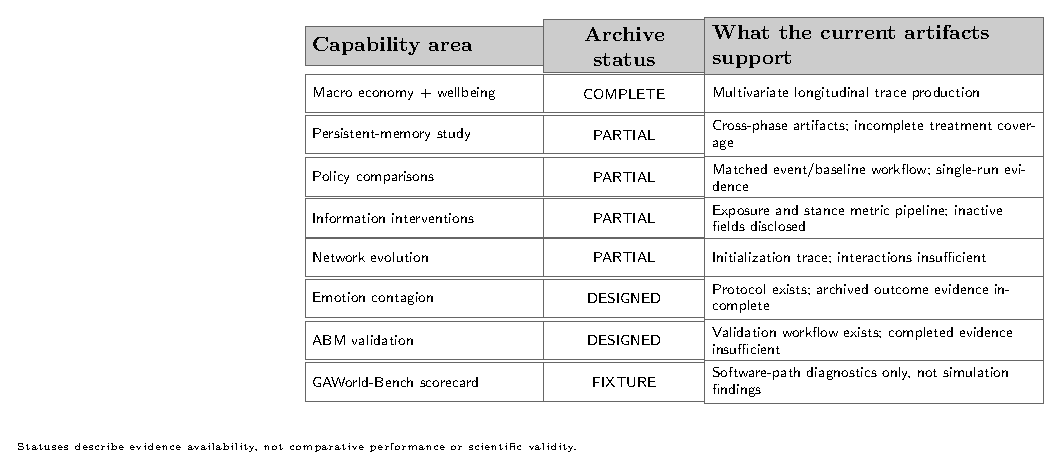
\includegraphics[width=\linewidth]{capability_matrix.pdf}
  \caption{Coverage of the audited result archive.  The matrix distinguishes
  inspectable capability evidence from incomplete evaluations and diagnostic
  fixtures; it is not a leaderboard or a validation score.}
  \label{fig:capability-matrix}
\end{figure}

\begin{table}[t]
\centering
\small
\caption{Status of all experiment families represented in the frozen artifact
ledger.  Counts and horizons describe the archived files, not a common
evaluation protocol.}
\label{tab:archive-status}
\begin{tabular}{@{}p{0.20\linewidth}p{0.16\linewidth}p{0.23\linewidth}p{0.33\linewidth}@{}}
\toprule
Area & Status & Archived scope & Permitted use \\
\midrule
Macro economy and wellbeing & Complete for description & $n=5$ agents, one seed, three-day configuration; 116 recorded steps per agent & Multivariate state-trace production, not an economic or psychological finding \\
Persistent memory & Partial & $n=1$ agent; four planned 14-day arms; only one completed both seven-day phases & Persistence and cross-phase artifact inspection, not a treatment comparison \\
Policy comparisons & Partial & Four single archived event--baseline pairs; Day-3 events; no seed replications & Pairing, isolation, and metric extraction, not policy effects \\
Information intervention & Partial & Three arms, $n=5$ each; unequal horizons of one or two days & Information-metric schema and missing/inactive-field audit \\
Polarization & Partial & Two arms with 109 versus 85 records & Availability of a comparison artifact; unequal records preclude an effect claim \\
Network evolution & Partial & $n=5$, 14-day report; zero recorded interactions on every day & Initialization and failure visibility, not emergent-network evidence \\
Emotion contagion & Designed / incomplete & Four intended arms; all four report a missing state-history file & Protocol coverage only; no outcome result \\
ABM validation & Designed / incomplete & Validation workflow is present; completed empirical evidence is insufficient & Evaluation design only, not an empirical validation result \\
GAWorld-Bench & Fixture & Built-in synthetic scorecard & Parser and scoring-path diagnostics only \\
\bottomrule
\end{tabular}
\end{table}

\subsection{Case 1: Persistence Is Observable, but the Memory Contrast Is Not}

The memory-consistency archive is useful because it exposes a longitudinal
experimental shape that is often hidden in agent demonstrations.  One agent
(ID 34) was assigned to four intended treatments: intact memory, reset between
phases, selective summary deletion, and injected conflict.  Each arm planned a
seven-day acquisition phase followed by a seven-day continuation phase.  The
archive contains seven phase-1 diaries for every arm, together with state and
memory files.  It also records different memory-file footprints, including
episodic, growth, habit, and relationship artifacts.  Thus a researcher can
inspect what persisted, what was deleted, and how a later elicited action was
represented.

Only the intact-memory arm, however, contains all seven phase-2 diaries.  The
reset, selective, and conflict arms each stop after phase 1, with the archived
report attributing the interruption to initialization after the worker pool
started.  The archive therefore demonstrates file-backed persistence across
two phases for one agent in one arm; it does not compare the behavioral effect
of memory retention, deletion, or conflict.  Qualitative labels such as a move
from ``procrastinating'' to ``active'' are post-hoc codings of a few generated
actions, not a validated continuity measure.  In particular, differences in
phase-1 final actions cannot explain missing phase-2 outcomes.  This failure is
scientifically informative at the infrastructure level: treatment completeness
must be checked before interpreting a fluent diary as longitudinal evidence.

\subsection{Case 2: Policy Artifacts Exercise a Counterfactual Workflow}

The policy archive contains four timestamped comparisons---traffic
restriction, housing subsidy, medical reimbursement, and job-training
subsidy.  Each stores an event arm beside a baseline arm and exports the same
metric columns, thereby exercising the isolation and reduction path described
in \cref{sec:experiment-workflow}.  All are single archived comparisons, with
events injected on simulation day 3 (09:00 for traffic and 08:00 for the other
three); there is no multi-seed sampling distribution or uncertainty estimate.

The raw CSV files also show why mechanistic inspection must precede substantive
interpretation.  In every pair, the final values of
\texttt{cross\_viewpoint\_exposure}, \texttt{misinformation\_risk},
\texttt{stance\_score}, and \texttt{toxicity\_score} are zero in both arms.
Some generic state variables differ: for example, the housing comparison has
a final event-minus-baseline \texttt{time\_pressure} difference of $-0.0311$
and the traffic comparison a \texttt{mobility\_intent} difference of
$-0.0036$.  These numbers are reported only to show that the reducer retains
metric direction and magnitude.  A single LLM-mediated trajectory cannot tell
whether the named policy caused the difference, whether the relevant
structural mechanism was connected, or whether the sign would persist under a
new seed.  The case supports a workflow claim---GAWorld can preserve paired
trees and compute declared contrasts---rather than a claim about housing,
health, training, or transport policy.

\subsection{Case 3: Information Metrics Make Inactivity Visible}

The misinformation artifact contains three five-agent arms.  The control and
treatment B each cover two simulated days, whereas treatment A covers one.
Across every recorded day and arm, average misinformation risk is $0.0$, and
the reported peak and final risks are also $0.0$.  Mean
cross-viewpoint-exposure is $0.06656$ for control, $0.06707$ for treatment A,
and $0.06635$ for treatment B.  The unequal horizons rule out a balanced
comparison, and differences at the fourth decimal place are descriptive
properties of these files, not estimated intervention effects.

That negative result is nevertheless a useful system diagnostic.  The archive
records treatment names, horizons, agent counts, daily risk series, and an
exposure aggregate together.  It does not prove that
misinformation propagated, that risk detection was sensitive, or that the
interventions changed exposure.  The separate polarization artifact reinforces
the boundary: its two arms contain 109 and 85 records, respectively, and thus
cannot be read as a balanced longitudinal contrast without reconstructing the
missingness.  GAWorld's value here is inspectability---inactive fields and
unequal coverage remain visible rather than being silently converted into a
success score.

\subsection{Case 4: Economy--Wellbeing Traces Provide Dense State, Not External Validity}

The macro-economy archive is the most complete artifact for demonstrating
multivariate trace production.  Its hashed long-format CSV contains 11,600
rows for five agents, 116 unique recorded steps per agent, and 20 metrics per
step ($5\times116\times20$).  The associated configuration describes a
three-day, seed-42 run.  Direct aggregation of the CSV gives 580 values for
each metric across agents and steps.  Mean emotion, stress, and economic
security are $0.4896$, $0.5490$, and $0.6270$, respectively; their observed
ranges are $[0.0233,0.9310]$, $[0.0907,0.9898]$, and
$[0.4455,0.8298]$.

The raw row count matters because the accompanying narrative report describes
``580 timesteps per agent.''  In the CSV, 580 is instead the number of
agent--step values for one metric ($5\times116$); each agent has 116 distinct
step identifiers.  We therefore use the CSV cardinalities rather than the
report's timestep wording.  This discrepancy illustrates the role of an
artifact ledger: even a plausible derived report must be checked against its
hashed source.

The trace can support new descriptive analyses without a new simulation.  For
example, partitioning the 116 step identifiers into consecutive ranges
$0$--$38$, $39$--$76$, and $77$--$115$ yields emotion means of $0.6365$,
$0.5020$, and $0.3305$, while stress means are $0.4122$, $0.5428$, and
$0.6916$.  These bins are equal-index summaries, not validated ``days,'' and
the trajectories remain generated state variables from one seed.  They show
that GAWorld records joinable, time-indexed state across agents and constructs;
they do not show human wellbeing dynamics, economic realism, or an effect of
any real-world shock.

\subsection{Failures Are Part of the Capability Record}

Two additional archives prevent the coverage matrix from becoming a showcase
of successful-looking outputs.  The network-evolution report describes five
nodes and two initialization edges over a nominal 14-day horizon, but records
zero agent--agent interactions on each of the 14 days; the edges were inferred
from initial co-location.  It cannot support a homophily or emergent-network
claim.  The emotion-contagion comparison contains four arm entries, all of
which report that their state-history CSV is missing.  It contains no contagion
outcome.  Finally, the GAWorld-Bench scorecard matches its built-in synthetic
fixture.  It verifies that parsers, checks, and report generation execute; it
is not a result from GAWorld agents.  Reporting these cases alongside the more
complete trace is essential to the scientific use of an inspectable system.

\section{Validation Boundaries}
\label{sec:validation-boundaries}

An artificial society is not validated by the realism of a transcript, by one
aggregate match, or by successful execution.  GAWorld separates five claim
levels: individual consistency, macro correspondence, emergent dynamics,
counterfactual response, and reproducibility.  Evidence at one level does not
compensate for absence at another.  This layered view follows established
agent-based-modeling practice in distinguishing implementation verification,
empirical validation, and the intended domain of use
\citep{grimm2006odd,windrum2007empirical,fagiolo2007critical}.

\begin{table}[t]
\centering
\small
\caption{Claim--evidence matrix for the audited GAWorld snapshot.  ``Current
support'' states the strongest defensible claim, not an aspirational goal.}
\label{tab:claim-evidence}
\begin{tabular}{@{}p{0.17\linewidth}p{0.28\linewidth}p{0.25\linewidth}p{0.22\linewidth}@{}}
\toprule
Claim level & Evidence required & Current support & Not established \\
\midrule
Individual consistency & Repeated independent elicitations; longitudinal and perturbation tests; external or held-out criteria & Persistent profiles, memories, diaries, interviews, and one completed two-phase arm are inspectable & Human fidelity, stable identity across models/seeds, or a memory-treatment effect \\
Macro correspondence & Pre-specified external targets; calibrated population; uncertainty and out-of-sample tests & State/economy pipelines can produce aggregates; benchmark fixtures test analysis code & Population representativeness, calibrated macro fit, forecasting, or real-city prediction \\
Emergent dynamics & Multiple seeds and scales; mechanism ablations; network/temporal diagnostics; robust qualitative patterns & Social and network mechanisms emit inspectable state; failures are archived & Polarization, contagion, homophily, or other stable emergent laws \\
Counterfactual response & Replicated randomized arms; verified intervention path; placebo and negative controls; uncertainty & Four paired event/baseline trees demonstrate comparison mechanics & Causal policy effects, sign stability, transportability, or welfare recommendations \\
Reproducibility & Immutable code/config/data/model snapshots; deterministic components; repeated reruns and failure accounting & Hashed result files, seeds/configs in some runs, file-backed traces, and a diagnostic harness & Bitwise replay of hosted LLM calls or complete end-to-end reproduction of every archive \\
\bottomrule
\end{tabular}
\end{table}

\subsection{Individual Consistency}

GAWorld implements the prerequisites for a consistency study: named persistent
agents, structured state, episodic files, recall, reflection, and longitudinal
logs.  These mechanisms allow within-agent questions such as whether a stated
preference survives intervening events or whether an interview answer is
traceable to stored experience.  The current memory case does not answer those
questions comparatively because three of four arms lack phase 2 and the only
complete arm contains one agent.  Generated behavioral coherence is also not
equivalent to correspondence with a real person.  A stronger evaluation would
repeat standardized probes before and after controlled memory perturbations,
separate temporal persistence from prompt sensitivity, and compare against
held-out observations where consent and provenance permit.

\subsection{Macro Correspondence}

Aggregating simulated variables is an implemented capability; calling the
aggregate realistic requires a separate calibration argument.  The audited
economy trace has five agents and one seed, while the benchmark scorecard is a
synthetic diagnostic fixture.  Neither represents a target population or
supports out-of-sample prediction.  Future macro validation should document
the sampling frame, map each simulated construct to an external measurement,
reserve targets for testing rather than calibration, and report uncertainty
across seeds and plausible parameterizations.  Agreement on a few marginal
means would remain insufficient if joint distributions, temporal patterns, or
subgroup errors failed.

\subsection{Emergence and Mechanism}

An emergent claim requires a pattern that is not merely written into a prompt
or initial condition and that recurs under controlled variation.  The present
archive does not meet that standard: the network study records no interactions,
the emotion study has no state files, and the polarization arms have unequal
record counts.  The existence of social-network, exposure, and affect fields
therefore establishes instrumentation, not a social law.  Appropriate tests
would vary population size and topology, ablate candidate mechanisms, quantify
between-seed variability, and trace a macro pattern back to micro-level events.
Where a field remains identically zero, the first question is whether the
mechanism and detector were active, not why society produced no effect.

\subsection{Counterfactual Validity}

The matched-run interface is a useful scaffold for counterfactual experiments,
but the archived policy differences are single contrasts produced by an
LLM-mediated dynamical system.  A common seed does not guarantee common latent
randomness after prompts diverge, and a policy description does not guarantee
that an economic or mobility mechanism changed.  Before interpreting a
difference, researchers should verify the intervention's path from event to
structural state, replicate both arms over seeds, pre-register target metrics,
and include placebo events or negative-control outcomes
\citep{lipsitch2010negative}.  External policy conclusions additionally require
a defensible mapping to the population and institutions of interest.  GAWorld
currently supports constructing and auditing such a study, not replacing it.

\subsection{Reproducibility as a Non-Compensatory Gate}

The artifact hashes used in this paper bind each numerical statement to an
audited byte sequence.  They do not bind the archive to a clean released
runtime: the audit began from a dirty working tree, and hosted providers may
change behavior independently of code, seed, or sampling parameters.  Missing
state files and interrupted arms further show that successful completion must
be recorded per treatment.  Consequently, a result that cannot be reconstructed
from code, configuration, inputs, model identity, and complete outputs should
not be promoted because it looks plausible or matches an external statistic.

For future releases, the minimum reproducibility unit should contain the exact
code revision plus a patch or clean tag, environment lockfile, initial
profiles and maps, provider/model identifiers, prompt and sampling settings,
random seeds, per-arm status, logs, and raw and derived artifacts.  Hosted-model
studies should estimate replay variability rather than promise bitwise
determinism.  The diagnostic benchmark can then serve as a regression gate:
fixtures test parsers and scoring logic, while separately labeled simulation
runs test whether scientific evidence has actually been produced.

\subsection{Intended Use}

At its present evidence level, GAWorld is best used for mechanism prototyping,
trace inspection, hypothesis generation, controlled software experiments, and
the design of more rigorous artificial-society studies.  The archive does not
support deploying GAWorld as a substitute population, forecasting real social
outcomes, ranking policies, or making decisions about identifiable people.
Those are not merely stronger wordings of the same result; they are different
claims requiring external data, identification, uncertainty quantification,
and governance that the current artifacts do not provide.

\section{Limitations, Ethics, and Roadmap}
\label{sec:limitations-ethics-roadmap}

GAWorld makes a broad set of mechanisms available in one runtime, but breadth
does not imply scientific validity or engineering completeness.  We separate
limitations of the current artifact archive, limitations of the system
implementation, and limitations inherent in representing social life through
LLM agents.  The resulting roadmap likewise separates engineering work that
improves the instrument from research work needed to justify substantive
claims.

\subsection{Evidence and reproducibility limitations}

The archived experiments are incomplete and heterogeneous.  Several contain a
single seed or one agent, treatment horizons differ, some mechanisms produced
identically zero fields, and some intended arms lack outcome files entirely.
The evidence ledger can make those conditions visible, but it cannot recover
missing treatments or provide statistical power after the fact.  The existing
cases therefore illustrate trace production, comparison mechanics, and
failure visibility rather than stable behavioral effects.  Claims about
individual consistency, macro correspondence, emergence, or counterfactual
response require purpose-built evaluation beyond the archive summarized here.

Reproducibility is also limited by model and provider dependence.  A seed does
not freeze a hosted model, its serving stack, safety filters, or routing
behavior.  Provider fallback may change the model used within a run; library,
prompt, or parser versions can change subsequent state; and concurrency can
alter call order.  Local models improve control but do not eliminate hardware,
runtime, and numerical variation.  Consequently, meaningful replication
requires more than source code and a seed: it requires resolved configuration,
prompt and sampling settings, provider and model identifiers, dependency
versions, active plugins, warnings, per-arm completion status, and raw
artifacts.  Hosted-model studies should measure replay variability rather than
promise bitwise determinism.

Runtime and monetary cost constrain the studies that can be performed.  A
persistent society may invoke generation, embedding, retrieval, reflection,
environment, and consolidation paths repeatedly across agents and ticks.
Model caching, rule-based fallbacks, configurable stages, and local providers
can reduce calls, but each changes experimental conditions.  Cost pressure can
also encourage small populations and short horizons that are inadequate for
emergence or uncertainty analysis.  Future evaluations should report call
counts, latency, failures, model routes, and estimated cost alongside simulated
scale and horizon.

\subsection{Architecture and data limitations}

The K1--K5 microkernel migration is complete for its defined scope, including
nine built-in plugins, movement validation, and audited standard interventions.
Compatibility paths nevertheless remain: memory, environment, and social
logic are not wholly plugin-owned, the Controller does not mediate every
action, and the Recorder is not the sole provenance stream.  Shared
dictionaries and the context escape hatch weaken schema enforcement and
ownership boundaries.
Third-party plugins run in process and should not be treated as sandboxed.  A
configured extension point therefore does not guarantee mechanism isolation,
security, or semantic equivalence under replacement.

The artifact layer has corresponding schema plurality.  Agent logs, long-form
state CSVs, environment timelines, memory stores, visualization traces,
economy audits, and plugin outputs use different schemas and sometimes
different notions of step or time.  This plurality preserves domain-specific
detail, but cross-subsystem analysis requires explicit joins and can silently
misread cardinality or missingness.  The discrepancy identified in the
economy case between report wording and raw CSV cardinality illustrates this
risk.  Until a versioned provenance schema and manifest bind clocks, entities,
mechanisms, and derivations, replay and analysis must remain artifact-aware.

Input profiles are another boundary.  They may be sparse, stylized,
synthetic, or assembled from data whose completeness and provenance vary.
Rich generated backstories do not repair missing observations; they can turn
uncertainty into plausible detail.  Profile coverage, source, consent,
transformation, and missingness should be documented, and downstream readers
should distinguish supplied attributes from model-generated elaboration.

\subsection{Ethical boundaries and affected communities}

Synthetic agents can create an illusion of access to perspectives that were
never actually observed.  Language models may reproduce stereotypes, suppress
within-group heterogeneity, and make marginalized identities appear more
uniform or legible than they are \citep{wang2025flatten}.  Conditioning a model
on demographic labels or a short profile does not confer lived experience,
community membership, consent, or authority.  Even when aggregate outputs
resemble survey responses in one setting, LLM agents should not be treated as
drop-in replacements for human participants \citep{dillion2023replace}.

GAWorld therefore must not substitute for engagement with people affected by
a research question or policy.  It cannot determine community priorities,
adjudicate contested values, estimate acceptable harms, or legitimate a
decision about housing, health, employment, policing, mobility, or information
governance.  For consequential applications, affected communities should help
define the question, categories, outcomes, unacceptable uses, and release
conditions; domain experts and empirical data are needed to evaluate whether
the modeled mechanisms correspond to the institutions at issue.  Simulation
may support deliberation or identify assumptions to test, but it cannot replace
participation, due process, or accountable public decision-making.

Profiles, memories, interviews, and generated social ties can also expose or
infer sensitive information.  Researchers should minimize collection, obtain
appropriate consent and permissions, separate identifiers from research
artifacts, restrict access, define retention and deletion policies, and assess
whether releasing prompts or traces could re-identify a source.  Dashboard,
relay, and environment services are local research tooling rather than
production-secure deployments; exposing them requires authentication,
encryption, authorization, audit, and abuse controls.  Generated claims about
real people should not be presented as observations, and simulated agents
should not be used to rank, target, or make decisions about identifiable
individuals.

\subsection{Engineering roadmap}

The engineering roadmap is to make current boundaries enforceable and current
artifacts easier to reconstruct.  Priorities are: (1) extend typed Controller
validation beyond movement where governance is required; (2) migrate remaining domain mechanisms incrementally behind declared
dependencies without changing their semantics silently; (3) replace shared
dictionary conventions with versioned schemas and explicit state ownership;
(4) unify trace identifiers and clock semantics through a manifest-backed
provenance layer while retaining domain-specific payloads; (5) capture model,
provider, prompt, fallback, dependency, and plugin resolution in every run;
and (6) add conformance, failure-injection, migration, security, and replay
tests.  These changes would improve composability and auditability.  They would
not, by themselves, validate an artificial society.

\subsection{Research roadmap}

The research roadmap begins only after the execution unit is reproducible.
For individual consistency, standardized repeated probes and controlled memory
perturbations should be evaluated against held-out criteria where consent and
provenance permit.  For macro correspondence, researchers should define a
sampling frame, map simulated constructs to external measures, separate
calibration from testing, and quantify subgroup error and uncertainty.  Claims
of emergence require multiple seeds, scales, topologies, and mechanism
ablations, with macro patterns traced to micro events.  Counterfactual studies
require verified intervention paths, replicated arms, pre-specified outcomes,
placebos or negative controls, and an explicit account of transportability.
Provider and prompt sensitivity should be treated as experimental factors, not
hidden implementation noise.

Finally, future studies should evaluate not only whether a simulated pattern
is reproducible, but also whether the representation and intended use are
appropriate.  Participatory problem formulation, impact assessment, and
documentation of excluded perspectives belong beside technical validation.
GAWorld's near-term role is therefore to make artificial-society hypotheses,
mechanisms, traces, and failures easier to construct and inspect---not to turn
generated populations into unearned evidence about society.


\bibliographystyle{plainnat}
\bibliography{references}

\end{document}
